
% VLDB template version of 2020-08-03 enhances the ACM template, version 1.7.0:
% https://www.acm.org/publications/proceedings-template
% The ACM Latex guide provides further information about the ACM template

\documentclass[sigconf, nonacm]{acmart}

\usepackage{tikz}
\usetikzlibrary{positioning, arrows.meta, fit, backgrounds, calc}
\usepackage{tabularx}
\usepackage{enumitem}
\setlength{\emergencystretch}{1em}

%% The following content must be adapted for the final version
% paper-specific
\newcommand\vldbdoi{XX.XX/XXX.XX}
\newcommand\vldbpages{XXX-XXX}
% issue-specific
\newcommand\vldbvolume{14}
\newcommand\vldbissue{1}
\newcommand\vldbyear{2020}
% should be fine as it is
\newcommand\vldbauthors{\authors}
\newcommand\vldbtitle{\shorttitle}
\newcommand{\minihead}[1]{{\noindent\textbf{#1.} }}
% leave empty if no availability url should be set
\newcommand\vldbavailabilityurl{URL_TO_YOUR_ARTIFACTS}
% whether page numbers should be shown or not, use 'plain' for review versions, 'empty' for camera ready
\newcommand\vldbpagestyle{plain}

\newcolumntype{Y}{>{\raggedright\arraybackslash}X}
\newcolumntype{P}[1]{>{\raggedright\arraybackslash}p{#1}}

\begin{document}
\title{CS6400-A Project Proposal (Group 4): Hybrid Retrieval with Budgeted Evidence Selection}

%%
%% The "author" command and its associated commands are used to define the authors and their affiliations.
\author{Navneet}
\affiliation{%
  \institution{Georgia Institute of Technology}
}
\email{n41@gatech.edu}

\author{Jigyasa Hasija}
\affiliation{%
  \institution{Georgia Institute of Technology}
}
\email{jhasija3@gatech.edu}

\author{Joseph Souaiby}
\affiliation{%
  \institution{Georgia Institute of Technology}
}
\email{jsouaiby3@gatech.edu}

\begin{abstract}
We will implement a RAG system with hybrid BM25 and dense retrieval, pairwise cross-encoder reranking, and section-aware evidence selection under a token budget. On identical chunks, we compare it with both required baselines on QASPER~\cite{dasigi2021qasper} and MuSiQue~\cite{trivedi2022musique}. Our original implementation and controlled ablations measure packed gold-evidence recall, reranking pool-size trade-offs, section affinity, and system cost. Retrieval makes no generative LLM calls; a fixed generator produces answers with provenance for supplementary QA evaluation. We report negative results as well as gains.
\end{abstract}

\maketitle

%% ---------------------------------------------------------------------------
\section{Introduction}

A Retrieval-Augmented Generation (RAG) system~\cite{lewis2020rag} answers a question in two stages: retrieval finds the passages most likely to contain the answer, and generation reads those passages and writes a response. On long documents such as research papers, the generator can only use what fits in its context, so retrieval quality should be judged on the \emph{packed} context under a token budget, not only on the ranked list~\cite{bala2026recall}.

\minihead{What is known} Hybrid BM25~\cite{robertson2009bm25} and dense~\cite{karpukhin2020dpr} retrieval can outperform either alone, and a tuned convex combination matches or beats RRF~\cite{cormack2009rrf, bruch2023fusion}. Cross-encoder reranking~\cite{nogueira2019bert} was the largest single gain on all three benchmarks of Singh et al.~\cite{singh2026beyond}, and BM25 interpolation can improve dense-retriever scores~\cite{wang2021interpolate}; this does not establish a benefit after cross-encoder reranking. Visconde reranks every paragraph of a QASPER paper~\cite{pereira2023visconde}. Most directly, Singh et al.~\cite{singh2026beyond} held a strong \emph{listwise} reranker fixed on QASPER and MuSiQue and found that rank fusion, RAPTOR-style hierarchy~\cite{sarthi2024raptor}, and graph expansion then add no reliable gain. Structure-aware methods retrieve larger units or neighbouring chunks~\cite{jiang2024longrag, llamaindexautomerge, langlois2026scar}. Budgeted packing has been studied with coverage objectives on multi-hop data~\cite{bala2026recall} and with context-budget diagnostics on QASPER~\cite{kim2026evidence}.

\minihead{The gap} Our study examines four connected questions for QASPER:
\begin{enumerate}[leftmargin=*,nosep]
  \item How much \emph{gold evidence} reaches the generator at a fixed token budget after each stage. Singh et al.~\cite{singh2026beyond} report ranking and answer metrics, including nDCG@10 and Success@10, but do not isolate paragraph-evidence survival through our budgeted packing stages.
  \item Whether their conclusion holds for a \emph{pairwise} cross-encoder and for weaker BM25 and MiniLM~\cite{minilmcard} first stages, both of which they explicitly leave to future work~\cite{singh2026beyond}.
  \item How small the reranking pool can be before evidence is lost.
  \item Whether section-aware selection still helps once a reranker has ordered the paragraphs~\cite{llamaindexautomerge, langlois2026scar}.
\end{enumerate}
QASPER's section structure~\cite{dasigi2021qasper} motivates testing section affinity. We will measure the proportion of multi-evidence questions and the degree of evidence co-location on dev before evaluating this hypothesis.

\minihead{What we do} We build the pipeline with every stage switchable, using the required baselines on identical chunks. We score each configuration by gold-evidence recall and all-evidence coverage of the packed context across budgets of 256--2048 tokens. We record candidate-pool misses and selection losses separately. For selection losses, logs retain score order, token costs, and the budget state to diagnose ordering and fit failures without asserting a causal partition. We ask three research questions:
\begin{itemize}[leftmargin=*]
  \item \textbf{RQ1 (first stage and pool).} How much gold evidence does each first stage (BM25, dense, RRF~\cite{cormack2009rrf}, convex~\cite{bruch2023fusion}) deliver to the packed context after pairwise reranking~\cite{nogueira2019bert}, and how small can the pool $N$ be before packed recall drops? Once every paragraph is scored, first-stage pool recall is no longer limiting; the pool-size trade-off is our focus.
  \item \textbf{RQ2 (selection).} At the same budget, does section-aware selection raise all-evidence coverage on multi-evidence questions over top-$k$ after reranking, and at what cost to single-evidence questions? We compare it against redundancy-aware selection~\cite{carbonell1998mmr, peng2025adagres, yu2026sfrag, matrixcontext}. On multi-hop Wikipedia data, coverage-based packing helps~\cite{bala2026recall}, but on QASPER a diversity penalty could exclude complementary evidence from one section. We test both possibilities.
  \item \textbf{RQ3 (features).} Do BM25 and dense scores still add to cross-encoder relevance as selector features? Prior work motivates fusion before reranking~\cite{wang2021interpolate}; whether these features help after reranking is an empirical question.
\end{itemize}
A negative answer to any question is a reportable result.

%% ---------------------------------------------------------------------------
\section{Proposed Approach}

The pipeline (\autoref{fig:pipeline}) retrieves broadly with a hybrid of BM25 and dense retrieval, scores candidates precisely with a cross-encoder, and then packs an evidence set into a fixed token budget. Every stage can be switched off; the required baselines are the first-stage boxes alone, packed with top-$k$.

\begin{figure*}[t]
\centering
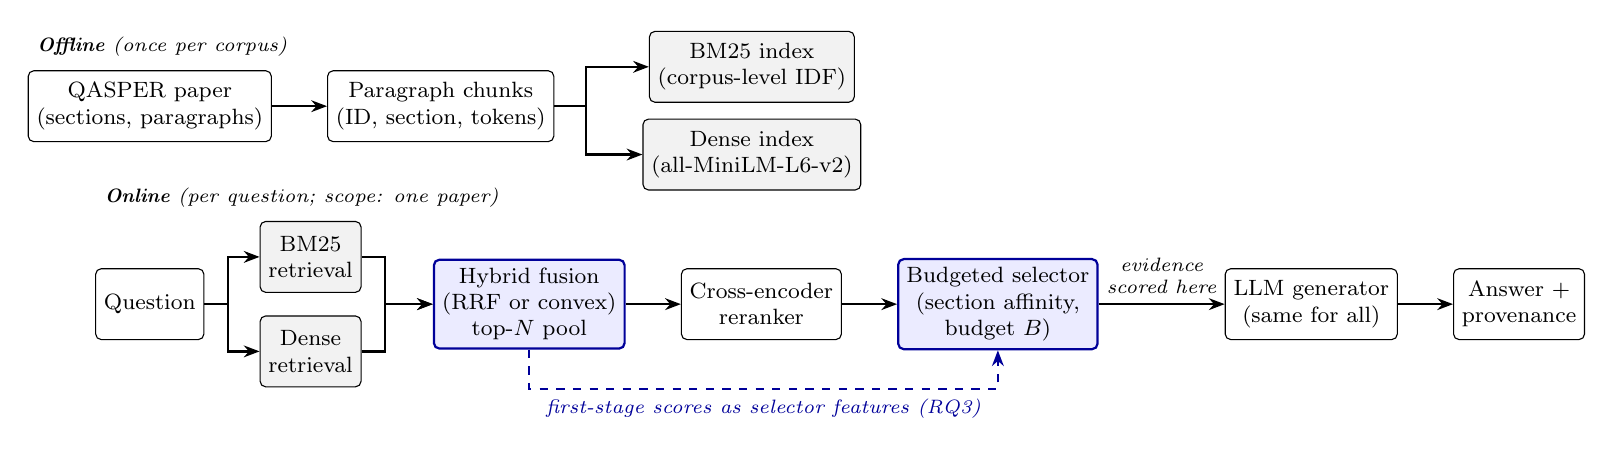
\begin{tikzpicture}[
    node distance=5mm and 7mm,
    box/.style={draw, rounded corners=2pt, align=center, font=\footnotesize, minimum height=9mm, inner sep=3pt, fill=white},
    ours/.style={box, fill=blue!8, draw=blue!60!black, thick},
    base/.style={box, fill=gray!10},
    arr/.style={-{Stealth[length=2mm]}, thick},
    darr/.style={-{Stealth[length=2mm]}, dashed, thick, blue!60!black},
    lbl/.style={font=\scriptsize\itshape, align=center}
  ]
  % offline row
  \node[box] (paper) {QASPER paper\\(sections, paragraphs)};
  \node[box, right=of paper] (chunk) {Paragraph chunks\\(ID, section, tokens)};
  \node[base, right=12mm of chunk, yshift=5mm] (bidx) {BM25 index\\(corpus-level IDF)};
  \node[base, below=2mm of bidx] (didx) {Dense index\\(all-MiniLM-L6-v2)};
  \draw[arr] (paper) -- (chunk);
  \draw[arr] (chunk.east) -- ++(4mm,0) |- (bidx.west);
  \draw[arr] (chunk.east) -- ++(4mm,0) |- (didx.west);

  % online row
  \node[box, below=16mm of paper] (q) {Question};
  \node[base, right=of q, yshift=6mm] (bm) {BM25\\retrieval};
  \node[base, right=of q, yshift=-6mm] (dn) {Dense\\retrieval};
  \node[ours, right=of q, xshift=22mm] (fuse) {Hybrid fusion\\(RRF or convex)\\top-$N$ pool};
  \node[box, right=of fuse] (ce) {Cross-encoder\\reranker};
  \node[ours, right=of ce] (sel) {Budgeted selector\\(section affinity,\\budget $B$)};
  \node[box, right=16mm of sel] (gen) {LLM generator\\(same for all)};
  \node[box, right=of gen] (ans) {Answer +\\provenance};

  \draw[arr] (q.east) -- ++(3mm,0) |- (bm.west);
  \draw[arr] (q.east) -- ++(3mm,0) |- (dn.west);
  \draw[arr] (bm.east) -- ++(3mm,0) |- (fuse.west);
  \draw[arr] (dn.east) -- ++(3mm,0) |- (fuse.west);
  \draw[arr] (fuse) -- (ce);
  \draw[arr] (ce) -- (sel);
  \draw[arr] (sel) -- node[lbl, above] {evidence\\scored here} (gen);
  \draw[arr] (gen) -- (ans);
  \draw[darr] (fuse.south) -- ++(0,-5mm) -| node[lbl, pos=0.25, below] {first-stage scores as selector features (RQ3)} (sel.south);
  \node[lbl, anchor=west] at ($(paper.north west)+(0,3mm)$) {\textbf{Offline} (once per corpus)};
  \node[lbl, anchor=west] at ($(q.north west)+(0,9mm)$) {\textbf{Online} (per question; scope: one paper)};
\end{tikzpicture}
\caption{System overview. Shaded blue boxes are the stages we contribute; gray boxes are the required baselines, which are evaluated alone with top-$k$ packing under the same budget. Gold-evidence recall is measured on the selector output, i.e., on what the generator actually receives.}
\label{fig:pipeline}
\end{figure*}

\subsection{End-to-End Design}

\minihead{Parsing} QASPER~\cite{dasigi2021qasper} ships each paper as a title, an abstract, and full text organized into named sections of paragraphs, plus figures, tables, questions, answers, and evidence annotations. We read this structure directly; no PDF parsing is needed.

\minihead{Chunking} One chunk is one paragraph, the same granularity as QASPER's gold evidence. Gold strings are matched exactly after Unicode and whitespace normalization. Unmatched evidence is retained as unreachable gold IDs in every method's denominator; no fuzzy matching is used. We canonicalize repeated normalized paragraphs and report ambiguous and unmatched evidence separately; no method uses test evidence in retrieval. Each chunk keeps a stable ID, its section title, and its token count.

\minihead{Indexing} We implement a BM25~\cite{robertson2009bm25} inverted index ourselves, and build a dense index of all-MiniLM-L6-v2~\cite{minilmcard, reimers2019sbert} embeddings with exact cosine search. MiniLM reads at most 256 wordpieces in its sentence-transformers configuration~\cite{minilmcard}, and may truncate long paragraphs. We report truncation rates for all paragraphs and gold paragraphs; every dense and hybrid configuration uses the same input limit and retains full source paragraphs for packing. For per-paper retrieval, BM25 IDF is computed over the training corpus rather than one paper, because term rarity inside a single paper of a few dozen paragraphs is a weak signal.

\minihead{Hybrid first stage} BM25 and dense rankings are fused by Reciprocal Rank Fusion~\cite{cormack2009rrf} (RRF) and, separately, by a convex combination of min-max normalized scores~\cite{bruch2023fusion}. The top $N$ candidates form the reranking pool; $N$ is an experimental variable. RRF uses $1/(60+\mathrm{rank})$ per channel. Constant-score channels normalize to zero; ties use stable source IDs.

\minihead{Cross-encoder reranking} We rerank with the pretrained cross-encoder bge-reranker-v2-m3~\cite{bgererankercard}, as a fixed off-the-shelf reranking component. It reads the question and each pooled paragraph together and outputs a relevance score, as in monoBERT reranking~\cite{nogueira2019bert}.

\minihead{Budgeted evidence selection} A greedy selector repeatedly adds the paragraph with the highest gain among those that still fit in the budget $B$, until no paragraph fits. For a candidate paragraph $p$ and the current selected set $S$, the gain is
\begin{equation}
\Delta(p \mid S) = R(p) + \mu\, n_S(\mathrm{sec}(p)).
\label{eq:gain}
\end{equation}
\begin{equation*}
R(p) = \alpha\, r_{\mathrm{ce}}(p) + \beta\, r_{\mathrm{bm25}}(p) + \gamma\, r_{\mathrm{dense}}(p),
\end{equation*}
We admit a candidate only if $c(S\cup\{p\})\leq B$. The $r$ terms are min-max normalized relevance scores over a fixed candidate pool, with $\alpha,\beta,\gamma\geq0$ and $\alpha+\beta+\gamma=1$. We count the serialized evidence text, source headers, and separators with the generator tokenizer and verify that the final context fits $B$. Fixed instructions and the question are counted separately in total prompt tokens. The count $n_S(\mathrm{sec}(p))$ is the number of already selected paragraphs from $p$'s supplied section (identified by its index, not just its title), and $\mu \ge 0$ is the section-affinity weight. Token cost is a budget constraint, not part of the score. Setting $\mu=0$ recovers ranking by $R(p)$ with budgeted packing: scan in score order, skip paragraphs that do not fit, and keep whole paragraphs. It recovers pure cross-encoder packing when $\alpha=1$ and $\beta=\gamma=0$. The section-affinity selector is a heuristic with no optimality guarantee. Exact paragraph IDs are kept for provenance. Similarity is embedding cosine, with an empty-set redundancy penalty of zero. All methods present selected paragraphs to the generator in source order.

\minihead{Why section affinity} It is structure-aware expansion at paragraph level, like merging chunks into parent sections~\cite{llamaindexautomerge} or retrieving larger units~\cite{jiang2024longrag, sarthi2024raptor}, but applied at selection time under a fixed budget, so it can be scored against gold paragraphs. We tune $\mu$ on dev with the cross-encoder in place and compare single- and multi-evidence questions. A zero affinity weight remains a valid choice if concentration does not help.

\minihead{Ablation rows} We keep two redundancy-aware selectors as ablation rows: relevance per token with max-similarity redundancy, $(R(p)-\lambda\max_{s\in S}\mathrm{sim}(p,s))/c(p)$, which adapts the packing scores of Matrix Context~\cite{matrixcontext} and SF-RAG~\cite{yu2026sfrag}; and maximal marginal relevance, $R(p)-\lambda\max_{s\in S}\mathrm{sim}(p,s)$~\cite{carbonell1998mmr}. These controls test whether length preference or redundancy penalties improve packed evidence recall. We do not stop adaptively: adding a feasible paragraph without displacing selected evidence cannot decrease evidence recall, although it may affect precision or answer quality, and min-max normalized scores offer no absolute threshold.

\minihead{Generation with provenance} The selected paragraphs are passed, with their IDs, to one fixed LLM (Qwen2.5-7B-Instruct~\cite{qwen25}). The system returns the answer together with the paper ID, section title, and exact text of every supplied paragraph. We request paragraph-ID citations and validate that cited IDs belong to the supplied context; this supplies provenance without assuming that citations prove correctness.

\subsection{Original Implementation}

We implement BM25 indexing, exact dense search, RRF and convex fusion, candidate-pool control, section-aware selection, and the evaluation harness. We reuse pretrained model inference and the official QASPER evaluator~\cite{dasigi2021qasper}; the packing trace is inspired by Matrix Context~\cite{matrixcontext}. The original harness implements mapping, budget checks, oracle ceilings, loss diagnostics, and paired statistics.

\subsection{Why We Expect Gains over the Baselines}

BM25 matches lexical identifiers, dense retrieval matches paraphrases, and fusion may recover complementary evidence~\cite{bruch2023fusion}. A cross-encoder can improve relevance ranking~\cite{nogueira2019bert}; section affinity tests whether evidence concentration adds value. Every budget table includes a gold-only oracle row. For each eligible annotation, it finds the largest feasible subset of mapped gold paragraphs under the same serialized token costs (by subset enumeration), then takes the maximum over annotations. Full-evidence feasibility is reported separately. Arbitrary gold-first ordering is not an optimal recall ceiling.

\subsection{Related Work}

The closest study is Singh et al.~\cite{singh2026beyond}, which uses our two benchmarks and asks whether retrieval add-ons help once a strong reranker is present. We extend it along the axes it leaves open: pairwise reranking, weaker first stages, the reranking pool size, gold evidence in the packed context, and the selection stage. Budgeted packing has been studied through context-budget diagnostics on QASPER~\cite{kim2026evidence} and coverage-based packing on multi-hop data~\cite{bala2026recall}. We add a stage-by-stage attribution and a structure-aware selector.

The overall pipeline shape (hybrid retrieval, reranking, budgeted greedy packing) already runs in Matrix Context~\cite{matrixcontext}. It uses one packer for all methods, on a synthetic benchmark at one budget; we borrow its trace of kept and dropped items for loss attribution. SF-RAG~\cite{yu2026sfrag} combines structure, reranking, and budgeted assembly on QASPER, but uses an LLM for section selection and also reports evidence F1 and structural diagnostics. Our distinction is the controlled first-stage/pool study, budget sweep, and lightweight section-affinity selector, rather than being the first to evaluate evidence-aware assembly. Agentic systems such as VecTree-RAG~\cite{zhong2026vectree} put an LLM inside retrieval; we do not.



%% ---------------------------------------------------------------------------
\section{Implementation Plan}

We write the pipeline in Python and reuse only pretrained models and generic numeric libraries; every retrieval, fusion, selection, and evaluation step is our own code. No RAG framework (LlamaIndex, LangChain) is used. \autoref{tab:impl} separates what we reuse from what we build.

\begin{table}[t]
  \caption{Components we reuse versus build.}
  \label{tab:impl}
  \footnotesize
  \begin{tabularx}{\columnwidth}{YP{1.5cm}Y}
    \toprule
    Component & Reuse / build & Tools \\
    \midrule
    Data loading, paragraph chunking, gold mapping & Build & Python; public QASPER and MuSiQue releases \\
    BM25 index and scoring & Build & Python inverted index, NumPy \\
    Dense embeddings & Reuse model; build index and search & sentence-transformers~\cite{reimers2019sbert}, all-MiniLM-L6-v2~\cite{minilmcard}, exact cosine in NumPy \\
    Hybrid fusion (RRF, convex) & Build & Python \\
    Cross-encoder reranking & Reuse model; build batching and pool logic & bge-reranker-v2-m3~\cite{bgererankercard} via Hugging Face Transformers \\
    Budgeted evidence selector & Build & Python, NumPy \\
    Generation with provenance & Reuse LLM; build prompt and citation output & vLLM~\cite{kwon2023vllm}, Qwen2.5-7B-Instruct~\cite{qwen25} \\
    Evaluation harness, per-stage loss trace, bootstrap statistics & Build; reuse F1 evaluator & Python, pandas; official QASPER evaluator~\cite{dasigi2021qasper} for answer and evidence F1 \\
    Latency and cost logging & Build & Python timers, scored pairs, prompt tokens, GPU runtime \\
    \bottomrule
  \end{tabularx}
\end{table}

\minihead{LLM access and use} We plan to serve Qwen2.5-7B-Instruct~\cite{qwen25} locally with vLLM~\cite{kwon2023vllm} on a compatible PACE ICE GPU, subject to allocation and a milestone feasibility check; one generator, one prompt, and greedy decoding are shared by every configuration. No LLM is used inside retrieval, which keeps retrieval cheap, deterministic, and comparable to the baselines.

%% ---------------------------------------------------------------------------
\section{Evaluation Plan}

Our primary metric is gold-evidence recall of the packed context at a fixed token budget, i.e.\ of what the generator actually receives, with answer quality and system cost reported alongside.

\subsection{Metrics of Success}

\autoref{tab:metrics} lists the metrics. For a question with a nonempty gold evidence set $G$ and selected set $S$ under budget $B$, evidence recall is $|S \cap G| / |G|$ and all-evidence coverage is 1 if $G \subseteq S$ and 0 otherwise, averaged over questions. QASPER questions often have several annotators with different evidence sets. We score against the best-matching annotator, as VecTree-RAG does~\cite{zhong2026vectree}. Because selecting the best annotator is optimistic, we always report union-of-annotators recall next to it. For paragraph retrieval, an eligible question has at least one answerable, nonempty, text-only evidence annotation. We report exclusions for unanswerable, empty-evidence, and figure/table-only cases, and score each metric against eligible annotations only. These are text-evidence subset metrics; full-task answer F1 includes unanswerables. Subgroups use the minimum deduplicated gold count across eligible annotations.

\begin{table}[t]
  \caption{Metrics we will report.}
  \label{tab:metrics}
  \footnotesize
  \begin{tabularx}{\columnwidth}{P{1.3cm}P{2.4cm}Y}
    \toprule
    Category & Metric & What it answers \\
    \midrule
    Retrieval (primary) & Evidence recall at budget $B$ & What fraction of gold paragraphs reached the packed context? \\
    Retrieval (primary) & All-evidence coverage at $B$ & Did every gold paragraph reach it? \\
    Retrieval & Evidence-F1~\cite{dasigi2021qasper} & Comparable with prior QASPER work \\
    Retrieval & Recall@$k$, MRR, nDCG@10 & Ranking quality before selection; nDCG@10 is comparable with Singh et al.~\cite{singh2026beyond} \\
    Retrieval & Oracle recall at $B$ & How much recall does the budget allow at all? \\
    Retrieval & Loss attribution & Was the missing evidence absent from the pool or lost during selection? \\
    QA (secondary) & Answer F1 (official QASPER evaluator); EM and F1 on MuSiQue & Does better evidence yield better answers? \\
    System & Scored question--paragraph pairs, p50/p95 latency, prompt tokens and GPU runtime & What does each gain cost? \\
    \bottomrule
  \end{tabularx}
\end{table}

\subsection{Benchmarks}

\minihead{QASPER (primary)} We follow QASPER's per-paper setting~\cite{dasigi2021qasper}: the paper is known and we retrieve among its paragraphs. An optional secondary pooled setting retrieves across all papers of the split; this is where first-stage recall limits everything downstream. We run it with and without the paper title prepended to each question, since the title alone can identify the paper, and report paper-level recall@$k$ separately.

\minihead{MuSiQue-Ans (secondary)} MuSiQue~\cite{trivedi2022musique} contains multi-hop questions whose context has 20 paragraphs, including annotated supporting paragraphs for each hop; each question needs 2 to 4 supporting paragraphs. Its 20-paragraph context mirrors QASPER's per-paper pool, and, as an optional extension, we build a deduplicated pooled corpus from the evaluation contexts to test the first stage at scale. This is our custom pooled setting, distinct from the supplied-context benchmark; we report corpus size and preserve supporting-paragraph IDs.

Metrics are supporting-paragraph recall and all-support coverage at budget $B$, plus answer EM and F1. Later-hop paragraphs are often reachable only through an earlier hop's answer. Because our retrieval is single-shot, we report recall per hop. On MuSiQue we run the RQ1 slice, which makes the comparison with Singh et al.~\cite{singh2026beyond} cover both of their homogeneous benchmarks.

\subsection{Evaluation Sets and Statistics}

\autoref{tab:evalsets} gives the splits. On QASPER we evaluate \emph{every} eligible test question; answer F1 uses a stratified subset and only BM25, dense, and the final proposed method at $B=1024$. MuSiQue QA uses 200 fixed questions from its retrieval evaluation sample. Both QA samples use a fixed seed and identical question IDs across methods.

Every method sees the same questions, so we compare methods with a paired bootstrap~\cite{efron1993bootstrap} that resamples papers (questions about one paper are correlated) and report 95\% confidence intervals. We resample QASPER papers and MuSiQue questions with 10,000 paired bootstrap replicates. We report effect sizes and 95\% intervals. Planned comparisons against both baselines and the cross-encoder-only packer use Holm correction within each benchmark; other grid comparisons are descriptive. Interval widths and eligible sample counts are measured rather than assumed. Full QASPER retrieval evaluation and 1,000 MuSiQue questions support paired comparisons; subgroup results may be less precise. We report subgroup counts (evidence count, answer type, hop count).

\begin{table}[t]
  \caption{Tuning and evaluation sets.}
  \label{tab:evalsets}
  \footnotesize
  \begin{tabularx}{\columnwidth}{P{1.3cm}YYY}
    \toprule
    Benchmark & Tuning set & Evaluation set & Selection \\
    \midrule
    QASPER & Dev split: 1,005 questions, 281 papers~\cite{dasigi2021qasper} & Test split: 1,451 questions, 416 papers~\cite{dasigi2021qasper}; all eligible questions & Full split for retrieval; 500 questions stratified by answer type for generation \\
    MuSiQue-Ans & 300 questions sampled from train & 1,000 of the 2,417 dev questions~\cite{trivedi2022musique} & Stratified by hop count (2, 3, 4) \\
    \bottomrule
  \end{tabularx}
\end{table}

% \subsection{Fair Comparison}

% Within each setting, all methods use identical paragraph chunks, corpus, and retrieval scope. Both required baselines are evaluated on both benchmarks, with generation on the same fixed QA samples. They are compared at the same token budget, counted with the generator's tokenizer, and the baselines are packed with top-$k$. We tune BM25 parameters and all hyperparameters (fusion weight, $\alpha,\beta,\gamma$, $\mu$, ablation $\lambda$) on the designated tuning sets for mean evidence recall across budgets; ties favor simpler settings. Final configurations and subgroup definitions are frozen before test evaluation, and test results are not used to revise them. Sampling seeds and selected question IDs are saved.

\subsection{Ablation Grid}

\autoref{tab:ablation} lists the axes. We run one slice per research question, not the full cross-product. \textbf{RQ1} crosses first stage with pool size at every budget, with top-$k$ packing. \textbf{RQ2} crosses selector with reranker on/off, budget, and evidence count, using the first stage selected on the tuning set from RQ1; the reranker-off cells isolate the selector without cross-encoder scores, using first-stage relevance with fixed dev-tuned settings. \textbf{RQ3} compares the two feature sets with the RQ2 selector fixed. We cache scores for each question--paragraph pair to replay quality ablations. Query-time latency runs bypass score caches, recompute query encoding and reranking with fixed batching, and count scored pairs for the actual pool $N$. Offline embedding/indexing cost is reported separately; cached replay time is not serving latency.

\begin{table}[t]
  \caption{Ablation grid.}
  \label{tab:ablation}
  \footnotesize
  \begin{tabularx}{\columnwidth}{P{2.2cm}Y}
    \toprule
    Axis & Values \\
    \midrule
    First stage & BM25, dense, hybrid RRF, hybrid convex \\
    Cross-encoder pool & 5, 10, 20, 30, whole paper (per-paper only); no reranker \\
    Selector & top-$k$ packing; section affinity (\autoref{eq:gain}); per-token redundancy and MMR (ablations) \\
    Selector features & cross-encoder only; cross-encoder + BM25 + dense \\
    Token budget & 256, 512, 1024, 2048 tokens \\
    Setting & per-paper (primary); pooled, with and without title \\
    \bottomrule
  \end{tabularx}
\end{table}

%% ---------------------------------------------------------------------------
\section{Timeline and Division of Work}

\minihead{By the milestone report} By W11, we will complete QASPER and MuSiQue loading, gold mapping, both retrieval baselines, hybrid fusion, and the evaluation harness with oracle and bootstrap. We will report dev-set evidence diagnostics and baseline results, and demonstrate vLLM serving with provenance on a small sample.

\minihead{By the final report (W16)} Cross-encoder reranking with pool control; the section-affinity selector and its ablations; the full grid on the QASPER test split in the per-paper setting; optional pooled experiments after the core evaluations; MuSiQue evaluation; answer F1 on the generation subsets with latency and cost; loss attribution, error analysis, and the final report.

\minihead{Division of work} Everyone runs ablations and writes their part of the report.
\begin{itemize}[leftmargin=*]
  \item \textbf{Navneet:} data loading, chunking, gold mapping, and the evaluation harness and statistics; also leads error analysis.
  \item \textbf{Jigyasa Hasija:} BM25, the dense index, hybrid fusion, and the cross-encoder pipeline; also runs the pooled-setting experiments.
  \item \textbf{Joseph Souaiby:} the budgeted selector, generation with provenance, and LLM serving; also handles latency and cost logging.
\end{itemize}

% \subsection{Risks and Mitigations}

% \begin{itemize}[leftmargin=*]
%   \item \textbf{The first stage stops mattering after whole-paper reranking}. Whole-paper scoring makes the candidate pool identical across first stages; this diagnostic measures the quality ceiling and scoring cost rather than a fusion gain. We report this as the RQ1 answer; the pool-size curve and the pooled setting still show where the first stage matters.
%   \item \textbf{The reranker already captures co-location}, leaving section affinity nothing to add. We report RQ2 as negative; the redundancy ablations still test whether set selection helps on QASPER.
%   \item \textbf{GPU limits on answer-F1 runs.} We use fixed generation subsets and check GPU feasibility by W11. If Ollama is needed, we freeze one checkpoint and precision before final runs and use that serving configuration for every method; the retrieval metrics do not depend on the LLM.
% \end{itemize}

\bibliographystyle{ACM-Reference-Format}
\bibliography{ref}

\end{document}
\endinput
